% % % % mainfile: ../../../../master.tex
\label{task:20240617_aosp}

\subsection{Why does debloating doesn't work anymore after relaunching?}

\subsubsection{Hyptothesis 1: Some thing is enabling JIT/AOT}

Find anything that's enabling compilation, like setting filter/profile to \texttt{speed} or \texttt{speed-profile} using:
\begin{lstlisting}[language=bash]
clear && find ./frameworks/ ./art/ ./bionic/ ./device/ ./build/ ./libnativehelper \( -iname '*.java' -o -iname '*.cpp' -o -iname '*.cc' -o -iname '*.hpp' -o -iname '*.h' -o -iname '*.S' -o -iname '*.mk' \) -a ! -iname '*test*' -a ! -iname '*out*' | xargs grep --color -sin 'speed-profile'
\end{lstlisting}

\subsubsection{Hypothesis 2: Understand the change in AOT/JIT process from AOSP 13 to 14}

Find anything changes related to JIT/AOT using:
\begin{lstlisting}[language=bash]
cd AOSP13\ vs\ AOSP14/
clear && find ./frameworks/ ./art/ ./bionic/ ./device/ ./build/ | xargs grep --color -sin 'jit'
\end{lstlisting}
I know that these files are only the files that have been touched by Zicheng. But we can start from here which has a relatively small search space.

\subsubsection{Check JIT Code Caching}

All procedures assocated with JIT:
\begin{longtable}{p{.45\linewidth}p{.55\linewidth}} 
\toprule
Procedure & Description \\
\midrule
\endhead

\multicolumn{2}{l}{\path{runtime/interpreter/interpreter.cc}}\\
\path{Execute}
&
\\

\multicolumn{2}{l}{\path{runtime/entrypoints/quick/quick_trampoline_entrypoints.cc}}\\
\path{artQuickGenericJniTrampoline}
&
\\

\multicolumn{2}{l}{\path{runtime/jit/jit.cc}}\\
\path{Jit::MethodEntered}
&
\\
\path{Jit::CompileMethod}
&
\\
\path{Jit::CompileMethodFromProfile}
&
\\
\path{JitCompileTask::Run}
&
\\
\path{Jit::CompileMethodInternal}
&
\\

\multicolumn{2}{l}{\path{compiler/jit/jit_compiler.cc}}\\
\path{JitCompiler::CompileMethod}
&
\\

\multicolumn{2}{l}{\path{compiler/optimizing/optimizing_compiler.cc}}\\
\path{OptimizingCompiler::JitCompile}
&
\\

\multicolumn{2}{l}{\path{runtime/jit/jit.cc}}\\
\path{JIT::MethodEntered}
&
\\

\multicolumn{2}{l}{\path{runtime/jit/jit-inl.h}}\\
\path{JIT::AddSamples}
&
\\

\multicolumn{2}{l}{\path{runtime/instrumentation.cc}}\\
\path{Instrumentation::BranchImpl}
& Inform listeners that a branch has been taken (only supported by the interpreter)
\\

\multicolumn{2}{l}{\path{runtime/instrumentation.h}}\\
\path{Branch}
& Inform listeners that a branch has been taken (only supported by the interpreter)
\\

\midrule
\caption{JIT Procedures} 
\label{tab:jitprocedures}
\end{longtable}

Found out that there's an entry from quick everytime the \texttt{ontextchange} is called:
\begin{lstlisting}
06-25 18:56:05.997  1373  2207 I putmethod.latin: [WEIMINN] quick_trampoline_entrypoints.cc::artQuickGenericJniTrampoline | Entered: void com.android.inputmethod.latin.BinaryDictionary.getSuggestionsNative(long, long, long, int[], int[], int[], int[], int[], int, int[], int[][], boolean[], int, int[], int[], int[], int[], int[], int[], float[])
06-25 18:56:05.998  1373  2207 I putmethod.latin: [WEIMINN] quick_trampoline_entrypoints.cc::artQuickGenericJniTrampoline | Entered: void com.android.inputmethod.latin.BinaryDictionary.getSuggestionsNative(long, long, long, int[], int[], int[], int[], int[], int, int[], int[][], boolean[], int, int[], int[], int[], int[], int[], int[], float[])
06-25 18:56:05.998  1373  2207 I putmethod.latin: [WEIMINN] quick_trampoline_entrypoints.cc::artQuickGenericJniTrampoline | Entered: boolean com.android.inputmethod.latin.BinaryDictionary.isCorruptedNative(long)
06-25 18:56:05.998  1373  2207 I putmethod.latin: [WEIMINN] quick_trampoline_entrypoints.cc::artQuickGenericJniTrampoline | Entered: void com.android.inputmethod.latin.BinaryDictionary.getSuggestionsNative(long, long, long, int[], int[], int[], int[], int[], int, int[], int[][], boolean[], int, int[], int[], int[], int[], int[], int[], float[])
06-25 18:56:05.998  1373  2207 I putmethod.latin: [WEIMINN] quick_trampoline_entrypoints.cc::artQuickGenericJniTrampoline | Entered: boolean com.android.inputmethod.latin.BinaryDictionary.isCorruptedNative(long)
\end{lstlisting}

Not compiled by JIT when instrumenting \texttt{JitCompiler::CompilerMethod}.

\subsubsection{Need to find the entry point of JIT and AOT invocations}



\subsection{Comprehensive Method Invocation Flow in AOSP 14}

\subsection{Comprehensive Code Compilation Flow in AOSP 14}

\subsection{Bionic Flow}

\subsection{Prepare Technical Document on Debloating}

\subsection{Learn Binder IPC Flow}

\subsection{Learn Package Manager Flow}

\subsection{Learn Permission Manager Flow}

% 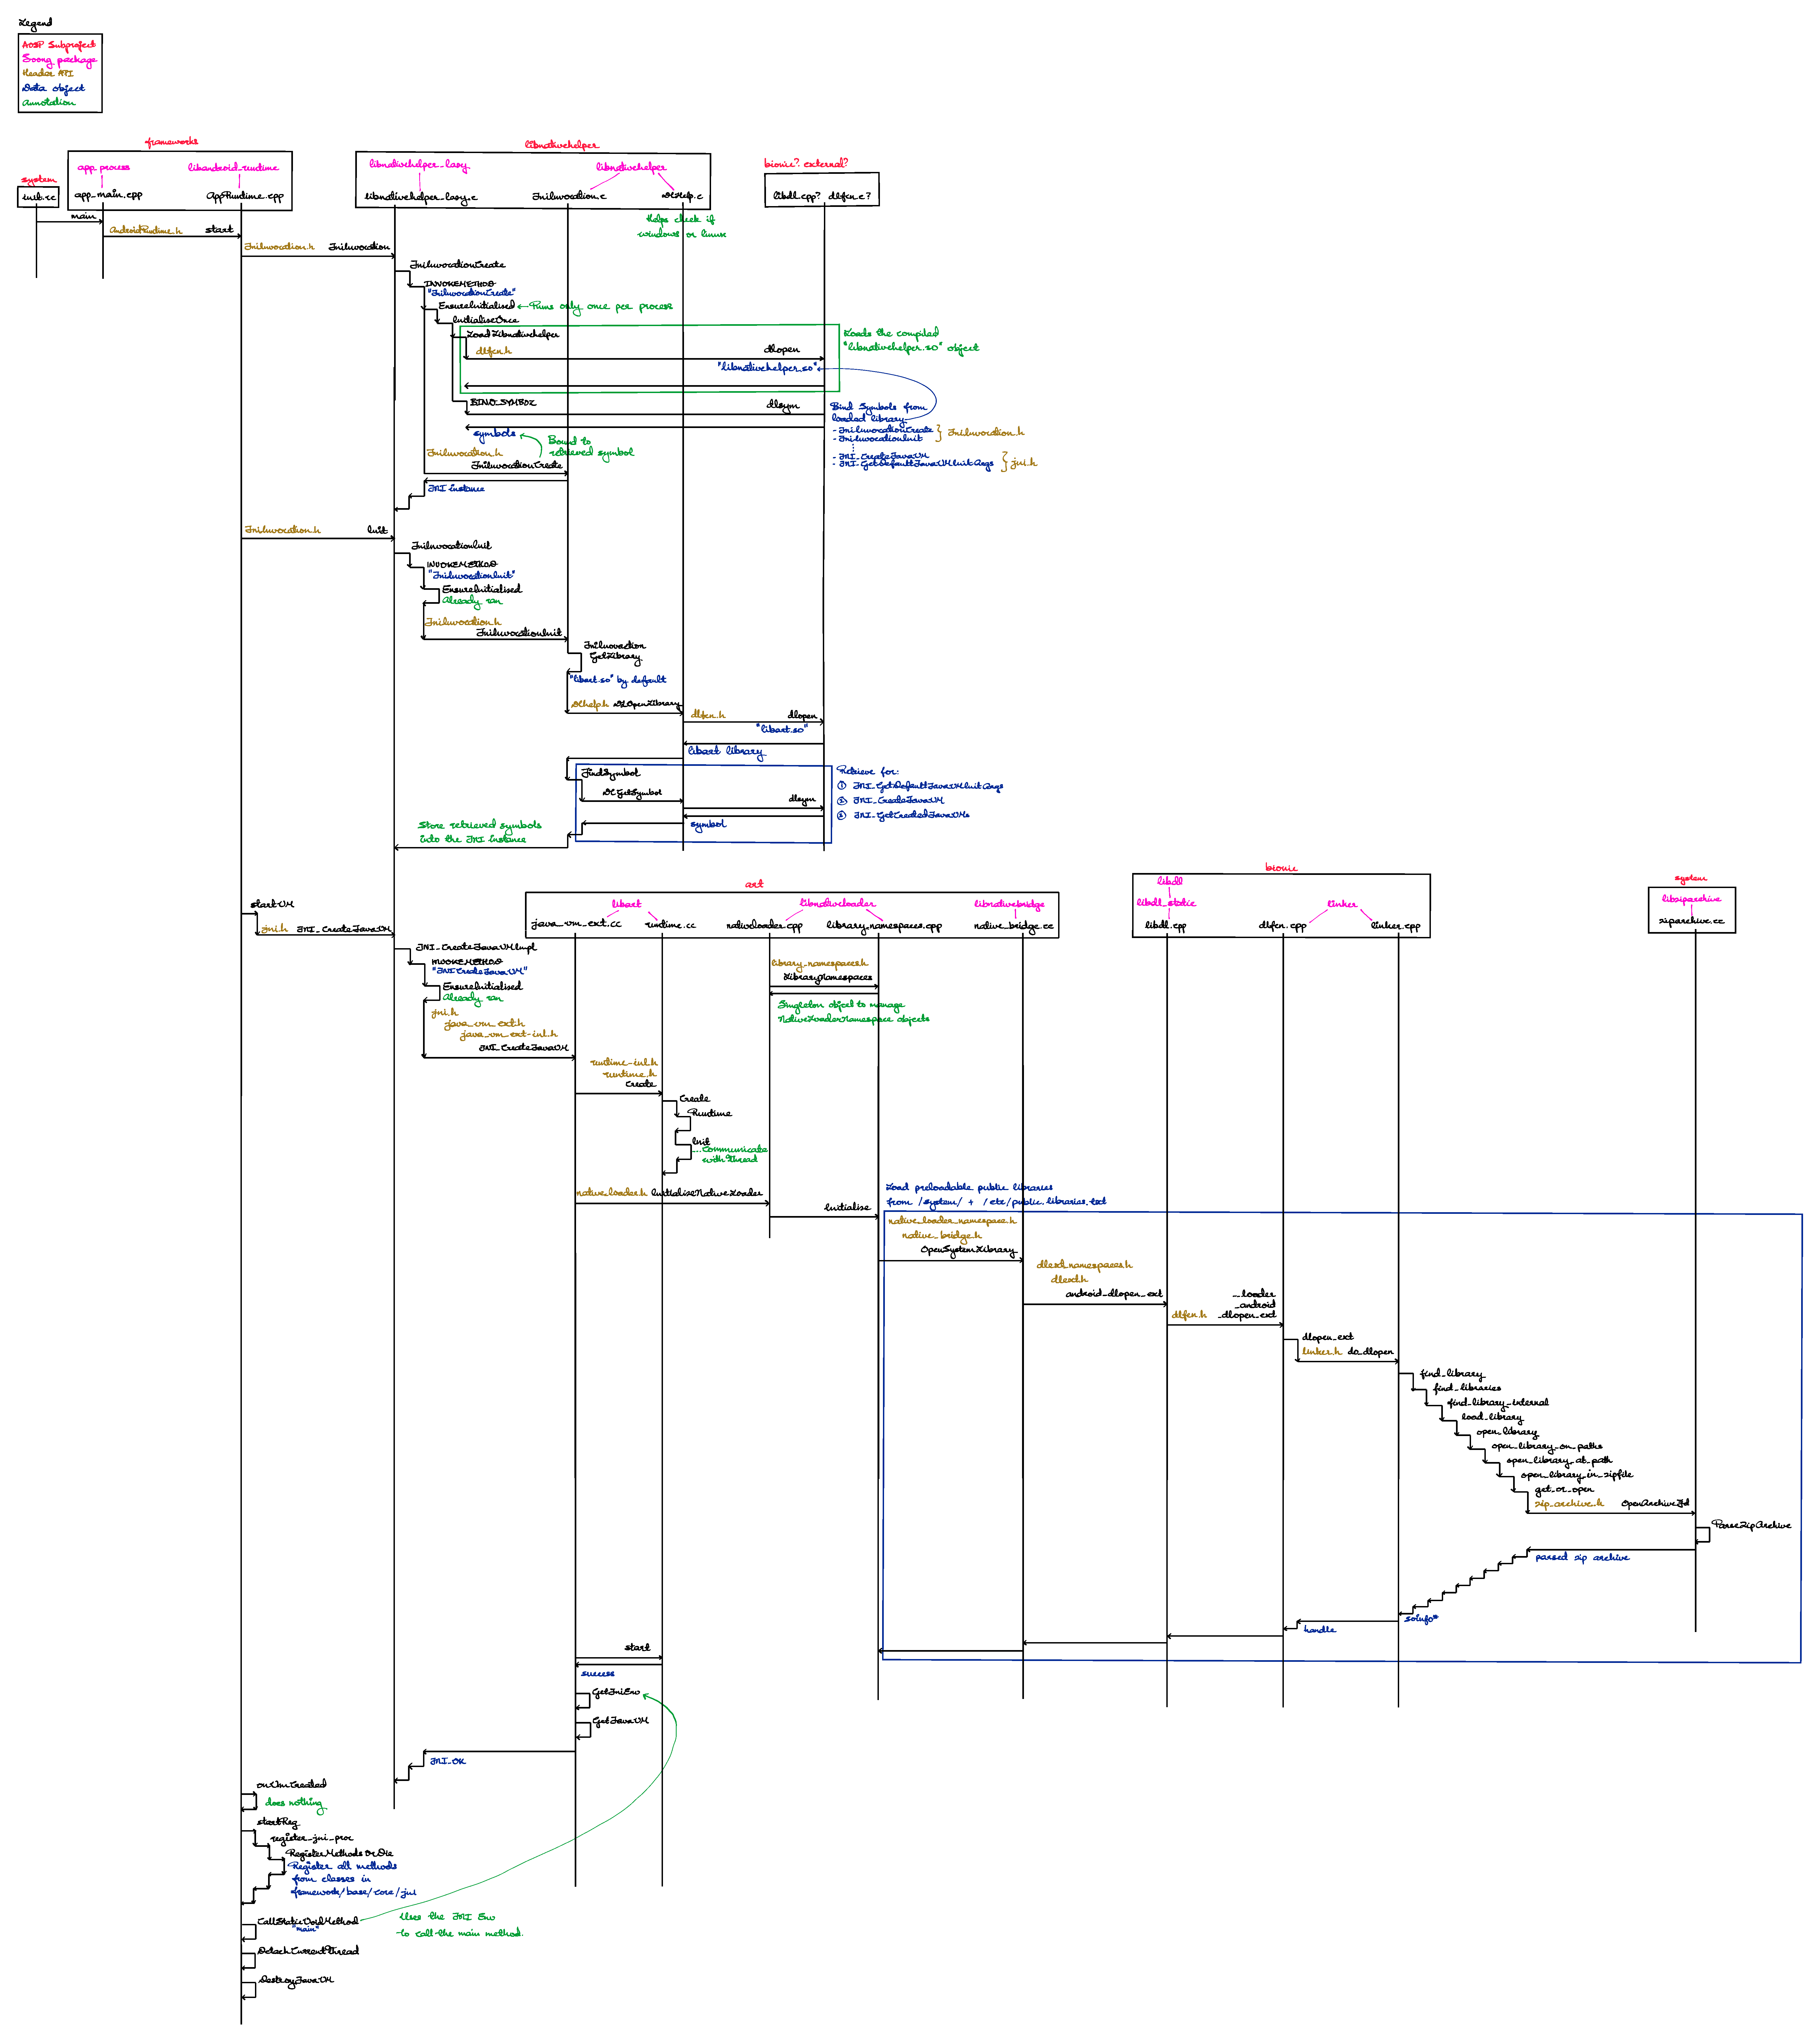
\includepdf[pages=-, scale=.95,pagecommand={}]{entries/2024/01/01/art.pdf}

% \begin{itemize}
% \item \textbf{Domain.} The context of the process that is acting upon something.
% \item \textbf{Type.} The context of the resource on which the process is acting.
% \item \textbf{Class.} The object class of the resource (e.g. \textit{file} or \textit{socket}).
% \item \textbf{Permissions.} The permissions that are allowed given the \textit{domain}, \textit{type} and \textit{class}.
% \end{itemize}

% SELinux rule syntax:


% \subsubsection{Decoding Permission Denial Message}

% Message:
% \begin{lstlisting}
% type=AVC msg=audit(1363289005.532:184): avc:  denied  { read } for  pid=29199 comm="Trace" 
% name="online" dev="sysfs" ino=30 scontext=staff_u:staff_r:googletalk_plugin_t 
% tcontext=system_u:object_r:sysfs_t tclass=file
% \end{lstlisting}

% \begin{longtable}{p{.15\linewidth}p{.15\linewidth}p{.65\linewidth}} 
% \toprule
% Log part & Name & Description \\
% \midrule
% \endhead

% \texttt{type=AVC}
% &Log type
% &Only in the \texttt{audit.log} file; it informs the user what kind of audit log type this is. 
% \\

% \midrule
% \caption{Permission Denied Syntax} 
% \label{tab:permissiondeniedsyntax}
% \end{longtable}


% \subsubsection{SELinux Architecture}

% SELinux consists of four main components: object managers (OM), access vector cache (AVC), security server, and security policy as show below:
% \begin{figure}[H]
%     \centering
%     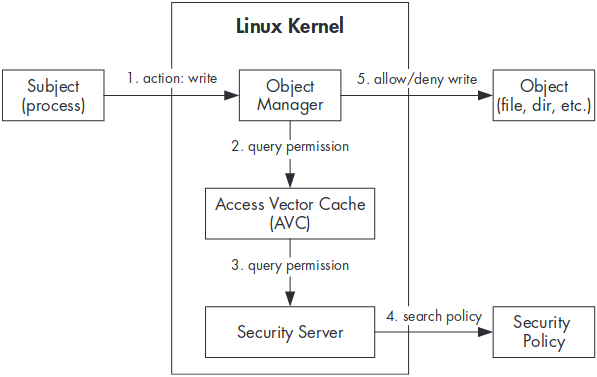
\includegraphics[width=.85\linewidth]{entries/2023/12/10/selinux.png}
%     \caption{SELinux Components}
%     \label{fig:selinux}
% \end{figure}
